\usepackage[utf8]{inputenc}
\usepackage{natbib}
\usepackage{times}
\usepackage[letterpaper, portrait, margin=1in]{geometry}
\usepackage{amsfonts}
\usepackage{amsthm}
\usepackage{amsmath}
\usepackage[dvipsnames]{xcolor}
\usepackage{siunitx}
\usepackage{amssymb}
\usepackage{graphicx}
\usepackage{mwe} % for blindtext and example-image-a in example
\usepackage{wrapfig}
\graphicspath{ {./images/} }
\usepackage{enumitem}
\usepackage{esvect}
\usepackage{tabto}
\usepackage[framemethod=TikZ]{mdframed}
\usepackage{mathtools}
\usepackage{braket}
\usepackage[scaled]{helvet}
\usepackage[T1]{fontenc}
\usepackage{framed}
\setcounter{section}{0}
\def \com{,\,}
\newtheorem{theorem}{Theorem}
\newtheorem{corollary}{Corollary}[theorem]

\newcounter{defn}[section]\setcounter{defn}{0}
\renewcommand{\thedefn}{\arabic{section}.\arabic{defn}}
\newenvironment{defn}[1][]{%
\refstepcounter{defn}%
\ifstrempty{#1}%
{\mdfsetup{%
frametitle={%
\tikz[baseline=(current bounding box.east),outer sep=0pt]
\node[anchor=east,rectangle,fill=blue!20]
{\strut Definition~\thelem};}}
}%
{\mdfsetup{%
frametitle={%
\tikz[baseline=(current bounding box.east),outer sep=0pt]
\node[anchor=east,rectangle,fill=blue!20]
{\strut Definition~\thedefn:~#1};}}%
}%
\mdfsetup{innertopmargin=10pt,linecolor=blue!20,%
linewidth=2pt,topline=true,%
frametitleaboveskip=\dimexpr-\ht\strutbox\relax
}
\begin{mdframed}[]\relax%
\label{#1}}{\end{mdframed}}

\newtheorem{lemma}[theorem]{Lemma}
\renewcommand\qedsymbol{$\blacksquare$}
\theoremstyle{remark}
\newtheorem{problem}{Problem}
\usepackage{lastpage}
\usepackage{fancyhdr} 
    \pagestyle{fancy}
    \fancyhf{}
    \rhead{Page \thepage \ of \pageref{LastPage}}
    \lhead{Problem Set \#1}
    
\newcommand{\dottedcolumn}[3]{%
  \settowidth{\dimen0}{$#1$}
  \settowidth{\dimen2}{$#2$}
  \ifdim\dimen2>\dimen0 \dimen0=\dimen2 \fi
  \begin{pmatrix}\,
    \vcenter{
      \kern.6ex
      \vbox to \dimexpr#1\normalbaselineskip-1.2ex{
        \hbox{$#2$}
    \kern3pt
    \xleaders\vbox{\hbox to \dimen0{\hss.\hss}\vskip4pt}\vfill
    \kern1pt
    \hbox{$#3$}
  }\kern.6ex}\,
  \end{pmatrix}
}

\usepackage{amssymb}
\usepackage[font={small, it}]{caption}
\usepackage{times}
\usepackage{hyperref}
\usepackage{ stmaryrd }

\usepackage{bm}
\usepackage{mathrsfs}

\usepackage[mathscr]{euscript}
% \usepackage{wasysym}
\usepackage{amsthm}
%\usepackage{pxfonts}
\usepackage[letterpaper, portrait, margin=1in]{geometry}
\usepackage{graphicx}
\usepackage{tikz}
\usepackage{tikz-3dplot}
\usepackage{pgfplots}
\usetikzlibrary{decorations.pathmorphing,patterns}
\usepackage{lipsum}
\usepackage{float}
\usepackage{subcaption}
\usepackage[object=vectorian]{pgfornament}
\usepackage{mwe}
\usepackage{bigints}
\usepackage{titlesec}
\setcounter{secnumdepth}{4}
\titleformat{\paragraph}
{\normalfont\normalsize\bfseries}{\theparagraph}{1em}{}
\titlespacing*{\paragraph}
{0pt}{3.25ex plus 1ex minus .2ex}{1.5ex plus .2ex}
\usepackage{mathtools}
\usepackage{pgfplots}
\pgfplotsset{compat=1.15}
\usepackage{lastpage}
\usepackage{enumitem}
\usepackage{tensor}
\usepackage{mathtools}
\usepackage{fancyhdr} 
    \pagestyle{fancy}
    \fancyhf{}
    \rhead{Page \thepage \ of \pageref{LastPage}}
\usepackage{setspace}
\usepackage{tikz}
\usetikzlibrary{hobby}

\usepackage{tikz-cd}

\theoremstyle{definition}

\newtheorem{thm}{Theorem}[section]
\newtheorem{example}[thm]{Example}
\newtheorem{lem}{Lemma}
\newtheorem{conj}[thm]{Conjecture}
\newtheorem{exc}[lem]{Exercise}
\newtheorem{fact}[thm]{Fact}
\newtheorem{claim}[thm]{Claim}
\newtheorem{corr}[thm]{Corollary}
\newtheorem{idea}[thm]{Idea}
\newtheorem{application}[thm]{Application}
\newenvironment{solution}
  {\renewcommand\qedsymbol{$\blacksquare$}\begin{proof}[Solution]}
  {\end{proof}}






%Short Cuts
    \renewcommand\qedsymbol{$\blacksquare$}
    \newcommand{\Pcal}{\mathcal{P}}
    \newcommand{\ve}{\varepsilon}
    \newcommand{\Ocal}{\mathcal{O}}
    \newcommand{\Amat}{\textsf{A}}
    \newcommand{\al}{\alpha}
    \newcommand{\be}{\beta}
    \newcommand{\Nbb}{\mathbb{N}}
    \newcommand{\Hbb}{\mathbb{H}}
    \DeclareMathOperator{\diag}{diag}
    \newcommand{\De}{\Delta}
    \newcommand{\Xcal}{\mathcal{X}}
    \newcommand{\Ga}{\Gamma}
    \newcommand{\Cscr}{\mathscr{C}}
    \newcommand{\Pbb}{\mathbb{P}}
    \newcommand{\B}{\mathbb{B}}
    \newcommand{\Dscr}{\mathscr{D}}
    \newcommand{\Efrak}{\mathfrak{E}}
    \newcommand{\Sbb}{\mathbb{S}}
    \newcommand{\La}{\Lambda}
    \newcommand{\de}{\delta}
    \DeclareMathOperator{\inte}{int}
    \newcommand{\Bscr}{\mathscr{B}}
    \newcommand{\Zscr}{\mathscr{Z}}
    \newcommand{\Xscr}{\mathscr{X}}
    \newcommand{\Escr}{\mathscr{E}}
    \newcommand{\Gscr}{\mathscr{G}}
    \newcommand{\om}{\omega}
    \newcommand{\gfrak}{\mathfrak{g}}
    \newcommand{\hfrak}{\mathfrak{h}}
   \newcommand{\kfrak}{\mathfrak{k}}
    \newcommand{\Om}{\Omega}
    \newcommand{\Fcal}{\mathcal{F}}
    \newcommand{\Oscr}{\mathscr{O}}
    \newcommand{\gl}{\mathfrak{gl}}
    \DeclareMathOperator{\Lie}{Lie}
    \DeclareMathOperator{\GL}{GL}
    \newcommand{\Xfrak}{\mathfrak{X}}
    \DeclareMathOperator{\id}{id}
    \DeclareMathOperator{\Int}{Int}
    \DeclareMathOperator{\End}{End}
    \DeclareMathOperator{\Aut}{Aut}
    \DeclareMathOperator{\stab}{stab}
    \DeclareMathOperator{\orb}{orb}
    \DeclareMathOperator{\grad}{grad}
    \DeclareMathOperator{\curl}{curl}
    \newcommand{\vp}{\varphi}
    \newcommand{\vt}{\vartheta}
    \DeclareMathOperator{\Gal}{Gal}
    \DeclareMathOperator{\rank}{rank}
    \DeclareMathOperator{\col}{col}
    \DeclareMathOperator{\Tame}{Tame}  
    \newcommand{\Yscr}{\mathscr{Y}}
    \newcommand{\Fbb}{\mathbb{F}}
    \newcommand{\arctanh}{\text{arctanh}}
    \newcommand{\pa}{\partial}
    \newcommand{\del}{\boldsymbol{\nabla}}
    \newcommand{\na}{\nabla}
    \newcommand{\Ycal}{\mathcal{Y}}
    \DeclareMathOperator{\spn}{span}
    \newcommand{\lap}{\nabla^2}
    \newcommand{\Pfrak}{\mathfrak{P}}
    \newcommand{\mfrak}{\mathfrak{m}}
    \newcommand{\Fvec}{\mathbf{F}}
    \newcommand{\Mcal}{\mathcal{M}}
    \newcommand{\ellvec}{\boldsymbol{\ell}}
    \newcommand{\rvec}{\mathbf{r}}
    \DeclareMathOperator{\supp}{supp}
    \newcommand{\Abb}{\mathbb{A}}
    \newcommand{\svec}{\mathbf{s}}
    \newcommand{\fs}{\vec{\sigma}}
    \newcommand{\bs}{\cev{\sigma}}
    \newcommand{\uvec}{\mathbf{u}}
    \newcommand{\iunit}{\boldsymbol{\hat{\i}}}
    \newcommand{\junit}{\boldsymbol{\hat{\j}}}
    \newcommand{\xunit}{\mathbf{\hat{x}}}
    \newcommand{\Char}{\text{char}}
    \newcommand{\kunit}{\mathbf{\hat{k}}}
    \newcommand{\theunit}{\boldsymbol{\hat{\theta}}}
    \newcommand{\pvec}{\mathbf{p}}
    \newcommand{\qvec}{\mathbf{q}}
    \newcommand{\yvec}{\mathbf{y}}
    \newcommand{\xvec}{\mathbf{x}}
    \newcommand{\wvec}{\mathbf{w}}
    \newcommand{\bvec}{\mathbf{b}}
    \newcommand{\Ucal}{\mathcal{U}}
    \newcommand{\Ncal}{\mathcal{N}}
    \newcommand{\Scal}{\mathcal{S}}
    \newcommand{\Nscr}{\mathscr{N}}
    \newcommand{\da}{\dagger}
    \newcommand{\CT}{\mathrm{H}}
    \newcommand{\Sscr}{\mathscr{S}}
    \DeclareMathOperator{\lcm}{lcm}
    \newcommand{\evec}{\mathbf{e}}
    \newcommand{\Kscr}{\mathscr{K}}
    \newcommand{\ebold}{\boldsymbol{e}}
    \newcommand{\zvec}{\mathbf{z}}
    \newcommand{\vvec}{\mathbf{v}}
    \newcommand{\Tscr}{\mathscr{T}}
    \newcommand{\avec}{\mathbf{a}}
    \newcommand{\Avec}{\mathbf{A}}
    \newcommand{\Ivec}{\mathbf{I}}
    \newcommand{\muvec}{\boldsymbol{\mu}}
    \newcommand{\Bvec}{\mathbf{B}}
    \newcommand{\Cvec}{\mathbf{C}}
    \newcommand{\eunit}{\mathbf{\hat{e}}}
    \newcommand{\vpunit}{\boldsymbol{\hat{\varphi}}}
    \newcommand{\zero}{\boldsymbol{0}}
    \newcommand{\tauvec}{\boldsymbol{\tau}}
    \newcommand{\runit}{\mathbf{\hat{r}}}
    \newcommand{\U}{\mathcal{U}}
    \newcommand{\Zbb}{\mathbb{Z}}
    \newcommand{\Bmat}{\textsf{B}}
    \newcommand{\Cmat}{\textsf{C}}
    \newcommand{\gmat}{\textsf{g}}
    \newcommand{\Ccal}{\mathcal{C}}
    \newcommand{\Rcal}{\mathcal{R}}
    \DeclareMathOperator{\Map}{Map}
    \DeclareMathOperator{\Frob}{Frob}
    \newcommand{\Imat}{\textsf{I}}
    \newcommand{\Rmat}{\textsf{R}}
    \DeclareMathOperator{\Frac}{Frac}
    \DeclareMathOperator{\Spec}{Spec}
    \DeclareMathOperator{\Emb}{Emb}
    \newcommand{\Kcal}{\mathcal{K}}
    \newcommand{\Wcal}{\mathcal{W}}
    \newcommand{\Lcal}{\mathcal{L}}
    \newcommand{\Tcal}{\mathcal{T}}
    \newcommand{\Ecal}{\mathcal{E}}
    \DeclareMathOperator{\im}{Im}
    \DeclareMathOperator{\nul}{Nul}
    \newcommand{\Qbb}{\mathbb{Q}}
    \newcommand{\ga}{\gamma}
    \newcommand{\la}{\lambda}
    \newcommand{\RomanNumeralCaps}[1]
        {\MakeUppercase{\romannumeral #1}} 
    \newcommand{\dif}{\text{d}}
    \newcommand{\Rbb}{\mathbb{R}}
    \newcommand{\Tbb}{\mathbb{T}}
    \DeclareMathOperator{\Hom}{Hom}
    \DeclareMathOperator{\conv}{conv}
    \newcommand{\Gr}{\text{Gr}}
    \newcommand{\Bcal}{\mathcal{B}}
    \newcommand{\Acal}{\mathcal{A}}
    \newcommand{\ddx}{\frac{d}{dx}}
    \newcommand{\pfrak}{\mathfrak{p}}
    \newcommand{\qfrak}{\mathfrak{q}}
    \newcommand{\Evec}{\mathbf{E}}
    \newcommand{\omvec}{\boldsymbol{\omega}}
    \newcommand{\alvec}{\boldsymbol{\alpha}}
    \newcommand{\gvec}{\mathbf{g}}
    \newcommand{\afrak}{\mathfrak{a}}
    \newcommand{\var}{\text{var}}
    \newcommand{\Cbb}{\mathbb{C}}
    \newcommand{\gavec}{\boldsymbol{\gamma}}
    \newcommand{\Tvec}{\mathbf{T}}
    \newcommand{\Vscr}{\mathscr{V}}
    \newcommand{\Ascr}{\mathscr{A}}
    \newcommand{\Uscr}{\mathscr{U}}
    \newcommand{\Sfrak}{\mathfrak{S}}
    \DeclareMathOperator{\sgn}{sgn}
    \DeclareMathOperator{\vol}{vol}
    \newcommand{\Pscr}{\mathscr{P}}
    \newcommand{\Wscr}{\mathscr{W}}
    \newcommand{\bcdot}{\boldsymbol{\cdot}}
    \DeclareMathOperator{\tr}{tr}
    \newcommand{\sectionline}{
        \noindent
        \begin{center}
        {
        {{
        {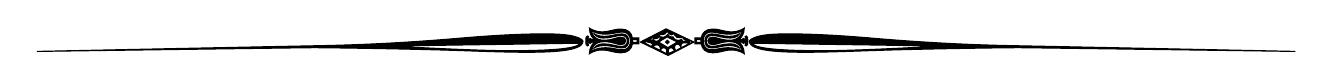
\begin{tikzpicture}
        \node  (C) at (0,0) {};
        \node (D) at (16,0) {};
        \path (C) to [ornament=89] (D);
        \end{tikzpicture}}}}}
        \end{center}
        }
    \newcommand{\sectionlineflip}{
        \noindent
        \begin{center}
        {
        {{
        {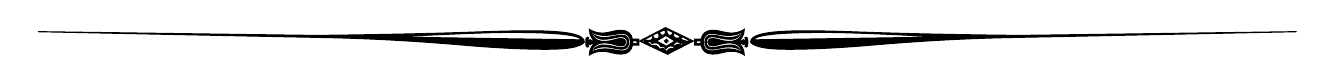
\begin{tikzpicture}
        \node  (C) at (0,0) {};
        \node (D) at (16,0) {};
        \path (D) to [ornament=89] (C);
        \end{tikzpicture}}}}} 
        \end{center}
        }
        
\makeatletter
\newcommand{\colim@}[2]{%
  \vtop{\m@th\ialign{##\cr
    \hfil$#1\operator@font colim$\hfil\cr
    \noalign{\nointerlineskip\kern1.5\ex@}#2\cr
    \noalign{\nointerlineskip\kern-\ex@}\cr}}%
}
\newcommand{\colim}{%
  \mathop{\mathpalette\colim@{\rightarrowfill@\scriptscriptstyle}}\nmlimits@
}
\renewcommand{\varinjlim}{%
  \mathop{\mathpalette\varlim@{\rightarrowfill@\scriptscriptstyle}}\nmlimits@
}
\renewcommand{\varprojlim}{%
  \mathop{\mathpalette\varlim@{\leftarrowfill@\scriptscriptstyle}}\nmlimits@
}

\newcommand{\goodemptyset}[1]{%
\begin{tikzpicture}[#1]%
\draw (0,0) circle (0.1);%
\draw(-0.07,-0.14)--(0.07,0.14);
\end{tikzpicture}%
}

\newcommand{\es}{\raisebox{-1pt}{\goodemptyset{}}}

\makeatletter
\DeclareRobustCommand{\cev}[1]{%
  {\mathpalette\do@cev{#1}}%
}
\newcommand{\do@cev}[2]{%
  \vbox{\offinterlineskip
    \sbox\z@{$\m@th#1 x$}%
    \ialign{##\cr
      \hidewidth\reflectbox{$\m@th#1\vec{}\mkern4mu$}\hidewidth\cr
      \noalign{\kern-\ht\z@}
      $\m@th#1#2$\cr
    }%
  }%
}
\makeatother

% bolding that isn't terrible
\newcommand{\vect}[1]{\mathbf{#1}}
\newcommand{\w}{\mathbf{w}}
\newcommand{\x}{\mathbf{x}}
\newcommand{\xalt}{\boldsymbol{\mathsf{x}}}
\newcommand{\y}{\mathbf{y}}
\renewcommand{\t}{\mathbf{t}}
\newcommand{\I}{\mathbf{I}}

% alternative variables
\newcommand{\xtilde}{\tilde{x}}
% custom math functions
\newcommand{\cov}{\mathrm{cov}}
\renewcommand{\var}{\mathrm{var}}
\newcommand{\E}{\mathrm{E}}
\renewcommand{\H}{\mathrm{H}}
\newcommand{\ML}{\mathrm{ML}}
% bad pictures
\newcommand{\centerimg}[2][3]{
\begin{center}
  \makebox[\textwidth]{\includegraphics[width=\paperwidth/#1]{#2}}
\end{center}
}
\newcommand{\sus}{\begin{tikzpicture}
    \draw (0,1) to[bend left=10] (0,6);
    \draw (0,1) to[bend right=5] (0,0);
    \draw (0,0) to[bend right=10] (2,0);
    \draw (2,0) to[bend right=5] (2.25,2);
    \draw (2.25,2) to[bend right=10] (3,2);
    \draw (1.75,2.125) to[bend right=8] (2.25,2);
    \draw (3,2) to[bend right=5] (3,-0.25);
    \draw (3,-0.25) to[bend right=10] (5,-0.25);
    \draw (5,-0.25) to[bend right=5] (5.25,7.25);
    \draw (5.25,7.25) to[bend right=30] (3,10);
    \draw (3,10) to[bend right=15] (2,10);
    \draw (2,10) to[bend right=30] (0.5,8.28);
    \draw (5.25,7.25) to[bend left=5] (6.25,7.15);
    \draw (6.25,7.15) to[bend left=5] (6.25,2.5);
    \draw (6.25,2.5) to[bend left=20] (5.25,2.25);
    \draw (-1,7.08) to[bend right=90] (3.25,7.08);
    \draw (-1,7.08) to[bend left=90] (3.25,7.08);
\end{tikzpicture}}
 
